%%%%%%%%%%%%%%%%%%%%%%%%%%%%%%%%%%%%%%%%%
% Simple Sectioned Essay Template
% LaTeX Template
%
% This template has been downloaded from:
% http://www.latextemplates.com
%
% Note:
% The \lipsum[#] commands throughout this template generate dummy text
% to fill the template out. These commands should all be removed when 
% writing essay content.
%
%%%%%%%%%%%%%%%%%%%%%%%%%%%%%%%%%%%%%%%%%

%----------------------------------------------------------------------------------------
%	PACKAGES AND OTHER DOCUMENT CONFIGURATIONS
%----------------------------------------------------------------------------------------

\documentclass[12pt]{article} % Default font size is 12pt, it can be changed here

\usepackage{geometry} % Required to change the page size to A4
\geometry{a4paper} % Set the page size to be A4 as opposed to the default US Letter

\usepackage{graphicx} % Required for including pictures

\usepackage{float} % Allows putting an [H] in \begin{figure} to specify the exact location of the figure
\usepackage{wrapfig} % Allows in-line images such as the example fish picture

\usepackage{lipsum} % Used for inserting dummy 'Lorem ipsum' text into the template

\linespread{1.2} % Line spacing

%\setlength\parindent{0pt} % Uncomment to remove all indentation from paragraphs

\graphicspath{{docs/}} % Specifies the directory where pictures are stored

\begin{document}

%----------------------------------------------------------------------------------------
%	INTRODUCTION
%----------------------------------------------------------------------------------------

\section{Background} % Major section



\begin{figure}[H] % Example image
\center{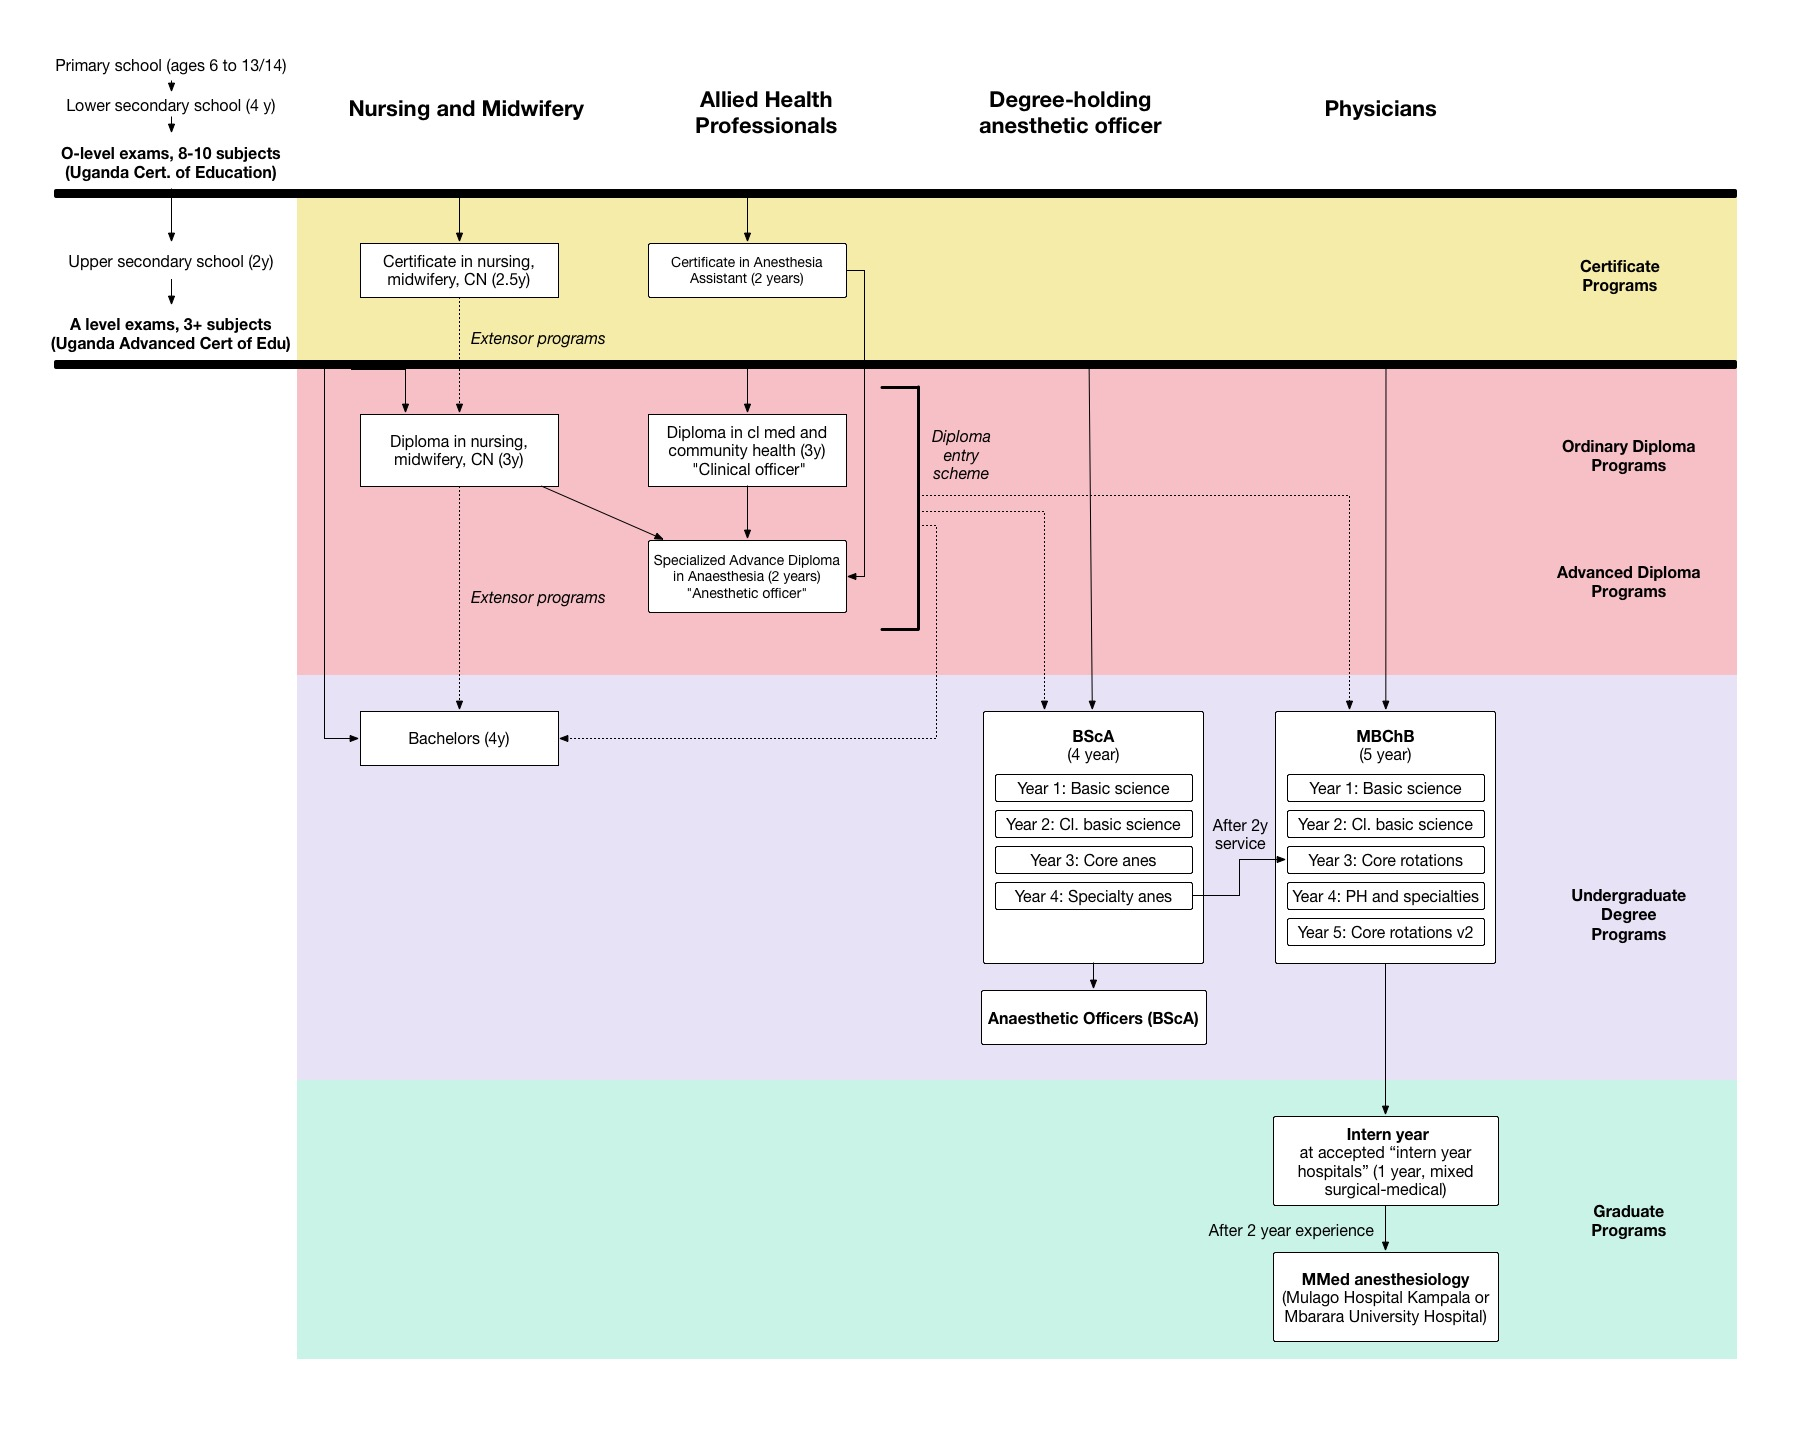
\includegraphics[width=1\linewidth]{training.jpg}}
\caption{Schematic of educational pathways}
\label{fig:edupathways}
\end{figure}

%----------------------------------------------
%	EDUCATION
%----------------------------------------------

\subsection{Education of anesthetists in Uganda} % Sub-section

\subsubsection{Secondary school and ordinary diploma programs}

After primary school, students in Uganda continue to a four-year program of lower secondary school, after which they take their first set of exams for the Ugandan Certificate of Education (UCE), also known as the ``O-level" exams. From here, they have the option of ending their secondary education and beginning career-focused training through certificate programs.  
\cite{UNFPA2009}
% Table R3 Analysis of curricula for different midwifery programmes. "O level 24 and A level is an added advantage"
In nursing, individuals can join certificate programs in nursing, midwifery, or comprehensive nursing (which combines portions of midwifery with traditional nursing). 
% new cadre eval 
These programs are 2.5 years and serve to build the minimum standards required for a community nurse at a health center. After completing one of such programs, individuals are referred to as ``enrolled nurses."
\cite{Klopper2012-pp}
% \cite{Klopper2012-pp}
% Table 22.5 lists programs and duration
% Can join without A-levels
% http://library.health.go.ug/download/file/fid/1376
% 5 Credits at O’ level in English, Mathematics Biology, Chemistry, Physics or Physical Science or General Science or Health Science
Alternatively, there is a 2-year certificate-level program in anesthesia at the Mbale School of Clinical Officers, after which one could join the workforce as an anesthetic assistant (AA). 
% Acorrding to the uganda allied health professionals council's registration list
% I'm not sure where I found that it was two years
% We don't have evidence this is still operating

Those individuals continuing to upper secondary school are able to sit for the Uganda Advanced Certificate of Education, or the "A-level" exams. Depending on the results, individuals may qualify to enter 3-year diploma programs in nursing or midwifery (to attain the title of ``registered nurse/midwife" or ``general nurse/midwife").
 \cite{Klopper2012-pp}
% Table 22.5 lists programs and duration
% Titiles from: http://library.health.go.ug/download/file/fid/1376
% There is conflicting information about whether A-levels are required. Older texts suggest they are not (\cite{UNFPA2009}), however many of the current admissions websites suggest they are. 
% I am not sure what differentiates "ordinary diplomas" from "advanced diplomas" or what the term "post-basic diploma" refers to (I assume same as 'advanced')
Alternatively, individuals can train as ``Clinical Officers." These individuals are integral to the functioning of district and regional hospitals, where their responsibilities include the assessment and treatment of patients. They can also perform minor procedures and assist in more complicated surgeries. This title is acquired through a 3-year diploma program in ``Clinical Medicine and Community Health." 
\cite{Banerjee2005Mar}
%To deal with the high demand for medical services in Uganda the post of a separate healthcare provider, termed a Medical Assistant, was developed in the 1960s. The title was officially changed to that of Clinical Officer (CO) in 1996. The qualification required to practise as a CO involves three years of training at specialist schools. The clinical work of COs initially comprised the diagnosis and treatment of patients in primary healthcare. The role has however expanded and today COs are also an integral part of district and regional hospitals. In the rural setting COs are responsible for the assessment, management and, where necessary, safe transfer of the surgical patient. In addition to their clinical work, COs are also often responsible for the administrative duties of their respective HCs. At the better-equipped Health Centres and District hospitals they undertake minor surgical procedures themselves and assist in more complex operations5.

All of the diploma-granting programs are also generally open to individuals who have completed certificate programs in relevant fields and who have spent multiple years in practice, and can enter without taking the A-level exams. This scheme is called ``extension" or ``mature entry."
% \cite{Klopper2012-pp}
% see table 22.4, available at refs/nursingentryreq.png 

\subsubsection{Anesthesia Officers}

Diploma-level training in anesthesia is available through an ``ordinary diploma" (leading to the designation of ``anesthetic assistant") or an ``advanced diploma," (also know as a ``post basic diploma") which requires a previous diploma. An advanced diploma confers a designation of ``anesthesia officer." 
\footnote{Many individuals currently registered with AHPC as AOs only appear to hold ordinary diploma}
\cite{dsco2012}
% \cite{dsco2012}
% This is the annoucement of vacacees and lists AA as needed "ordinary diploma" and "adv diploma" for AO
% This school lists AA=ordinary diploma http://mambosms.ug/Data/atha/lacorh/?page_id=7346
Little is published concerning the structure of these training programs.

As of March 2018, diploma level training is available at seven programs: Uganda Allied Health Institute and Management Sciences-Mulago (formerly Paramedical Training
schools), Mbale School of Clinical Officers, Fort Portal School of Clinical Officers, Lacor School of Anesthesia, Gulu School of Clinical Officers,  Ishaka Adventists Anaesthetic Officer Training School, Kitovu Catholic Anaesthetic Officer Training School. 
\cite{mohscholar2017}
Uganda Allied Health Institute and Management Sciences is the largest training program and has trained the vast majority of registered AOs in the nation. It offers a 2-year advanced program. 
\cite{mugalopara2013}
% See the registration DB
Lacor offers a 2-year Advanced Diploma in Anesthesia. It trains about 25 students a year and is associated with the Uganda Allied Health Institute and Management Sciences.
\cite{lacoranes2018}
%The School of Anaesthesia, on the other hand, is a Government school belonging to the Uganda institutes of Allied Health and Management Sciences, Mulago Kampala. The School of Anaesthesia was started in 1997, in response to increased surgical interventions and relatively limited numbers of anaesthesiologists to manage emergencies and elective surgical procedures. This is a pilot centre for students from the Northern Region who wish to study Anaesthesia. We have so far trained 24 Anaesthetic Officers and 58 Anaesthetic Assistants providing anaesthetic services in government and non- government institutions in Uganda. Generally, we have 25 Anaesthetic Officers under training. We are dedicated to improving anaesthetic services through our production units and ensuring that all regional referral hospitals and HCVI have trained anaesthetists.
Gulu offers a 2-year Advanced Diploma in Anesthesia.
% https://www.newvision.co.ug/new_vision/news/1449260/notice-gulu-school-clinical-officers
There is little-to-no published information about the programs at Mbale, Fort Portal, Ishaka Adventist or Kitovu Catholic.
% Mugalo and Mbale have problems.
% Uganda: The Mess At Mulago Paramedical School
% John Semakula and Jessica Nawati 
% http://allafrica.com/stories/201212170025.html
% https://www.newvision.co.ug/new_vision/news/1312882/suspended-mulago-paramedical-students-miss-exams
% Only 4 tutors? http://www.monitor.co.ug/News/National/Mbale-clinical-school-has-only-four-tutors/688334-2968568-8kilwp/index.html 
% https://ugandaradionetwork.com/story/mbale-clinical-school-administrators-investigated

Registration of all allied health professionals, including anesthetic officers, is managed by the Allied Health Professional Council (AHPC). As of 2016, only two anesthesia training programs were recognized by the council: UIAHMS and the Gulu School of Clinical Officers. 

An national exam is administered for graduates of the advanced diploma in anesthesia. The exam is administered by the Uganda Allied Health Examinations Board (UAHEB), which currently only recognized three AO training programs: Uganda Allied Health Institute and Management Sciences, Mbale School of Clinical Officers, and the Fort Portal School of Clinical Officers
\cite{examboardschools}
In 2014 and 2015, there was a 90\%  (n=26) and 100.00\% (n=17) pass rate for anesthesia boards, respectively.
\cite{examboard2015}

Depending on the results of A-level exams (generally, two principal passes), a secondary school graduate may qualify for entrance into degree-granting bachelor's programs in nursing, medicine, or a newly-formed Bachelor of Anesthesia. Alternatively, individuals may enter bachelor-level programs with poorer performance on the A-level exams (ie, one principle pass) if they already hold a diploma in a relevant field. This is referred to as a ``diploma entry" scheme.
\cite{mak2018}

A new four-year training program developed at Butesema University offers a Bachelor of Science in Anesthesia (BScA). Admission to this program requires either university-qualifying performance on A-level exams or a previous diploma in nursing, midwifery, or anesthesia. Students will complete two years of basic science education with their physician (MBChB) counterparts, then complete two years of anesthesia, critical care, and pain management training. After completion of their BScA, they will have the option to join the third-year of the MBChB program after required service.
\cite{aau2018}

\subsubsection{Physician Anesthetists}

Physicians hold the degree of MBChB after completion of a 5-year training program. Admission to MBChB programs, similarly to other bachelor-degree programs, can be obtained directly after secondary school, or alternatively, through a diploma entry scheme. \footnote{Some MBChB programs, such as Makerere, do not offer diploma-entry schemes for the MBChB} After the MBChB is granted, physicians join a one-year internship (comprised of mixed medical and surgical training) at an internship-approved hospital.
\cite{must2014}
Specialty training in anesthesia is obtained through a Master of Medicine in Anesthesia degree, a two-year program which requires completion of an internship year and two years of physician experience. There are two such programs: Mulago Hospital Kampala (associated with Makerere univerity) and Mbarara University Hospital of the Mbarara University of Science and Technology.


%----------------------------------------------
%	FACILITIES
%----------------------------------------------

\subsection{Facilities} % Sub-section

Uganda is divided into administrative units as follows (descending population): Districts, Counties, Consitituencies, Sub-Counties, Parishes and Villages. 
% \cite{UBS2017}
% "Uganda is stratified into administrative units namely; Districts, Counties, Consitituencies, Sub-Counties, Parishes and Villages to facilitate service delivery nearer to the people." Page 1 
There are 122 districts, 255 counties, 296 constituencies, 1460 sub-Counties, and 7467 parishes. There are new districts. Namisindwa, Pakwach, Butebo, Rukiga, Kyotera, and Bunyangabu districts were created July 1 2017. Much of the data we utilized was from before this change. Kagadi, Kakumiro, and Rubanda were created from the Kabaale district in 2016. Omoro was created from the Gulu district in 2016.
% \cite{UBS2017}
% "In total, there are 122 districts as at 1 st July 2017, including Kampala Capital City. Below is a table indicating the number of administrative units at lower levels by region." Page 1

Health facilities are divided into hospitals and health centers. Health centers are divided into four designations, Health Center I (mostly referred to as a "clinic") through Health Center IV. \cite{UBS2017}
% \cite{UBS2017}
% "Health facilities in Uganda include hospitals and health centres (IV, III and II). The number of functional healthcare facilities in 2015/16 was 5,117 down from 5,205 that were registered in 2012/13 as shown in Table 2.5.1 below." Page 43


There are two national hospitals (Mulago and Butabika Psychiatriac Hospital), four regional referral hospitals, and 139 district, or general, hospitals. Of these, 65 are government owned, 63 are owned by non-profits and 27 are private for-profits.
\cite{MOH-hosp-list}
% \cite{MOH-hosp-list}
%The total number of hospitals (public and private) in Uganda is 155. Of these 2 are National Referral Hospitals (Mulago and Butabika) , 14 are Regional Referral Hospitals (RRHs) and 139 are General Hospitals (GHs). In terms of ownership, 65 are government owned , 63 PNFP and 27 are private. Hospitals are major contributors to outputs of essential clinical care and take up a large volume of human and financial resources. In the financial year 2014 /15 almost similar to the year before, hospitals produced 54% of all inpatient admissions, 19% of total outpatients, and 36% of all deliveries. There are 139 GHs in the country providing; preventive, promotive outpatient curative, maternity, inpatient, emergency surgery and blood transfusion and laboratory services.
In total, in 2015/16, there were 2,932 government-run health facilities, 983 NGO-run, and 1202 privately-operated facilities.
% \cite{UBS2017}
% Table 2.5.1,  Source: Ministry of Health, HMIS 2015/16
Health center II’s are simple outpatient treatment centers which should be staffed by an enrolled nurse, working with a midwife, two nursing assistants and a health assistant. By law, each parish should have at least one functioning health center II. 
% \cite{UBS2017}
% "Out-patient clinic treating common diseases and offering antenatal care. It is supposed to be led by an enrolled nurse, working with a midwife, two nursing assistants and a health assistant. According to the Ugandan government's health policy, every parish is supposed to have a Health Centre II." (Page XX)
Health center III’s are managed by a clinical officer and should include an operating theatre for minor surgeries and cesarean section. Health center IV’s should have a physician on staff, separate wards for men, women, and children, as well as a operating theatre for emergency surgery.
% \cite{UBS2017}
% Health centre with facilities which include an operation room and a section for minor surgery. It is headed by a clinical officer, offers the continuous basic preventive and curative care and provides support supervision of the community and the Health Centre II facilities under its jurisdiction. According to the Ugandan government's health policy, every sub-county is supposed to have a Health Centre III. IV: A mini-hospital that provides the kind of services found at Health Centre III, but in addition has separate wards for men, women, and children in which to admit patients. It should have a senior medical officer and another doctor as well as a theatre for carrying out emergency operations. According to the Ugandan government's health policy, every county or parliamentary constituency is supposed to have a Health Centre IV." (Page XX)
District hospitals (also known as ``general hospitals") include all the services of Health Center IVs, as well as blood transfusions.
% \cite{UBS2017}
% General hospitals: Health facilities that provide preventive, outpatient curative, maternity, inpatient health services, emergency surgery, blood transfusion, laboratory and other general services. They also provide in-service training, consultation and research in support of community-based health care programmes.
Regional referral hospitals include additional specialized services such as radiology, pathology, and surgical sub specialties.
%In addition to the services offered at the general hospital, these hospitals offer specialist services such as psychiatry, ear, nose and throat, radiology, pathology, ophthalmology as well as higher level surgical and medical services, including teaching and research.
Finally, the national referral hospitals offer comprehensive specialist services. 
%In addition to the services offered at the regional referral hospital, they provide comprehensive specialist services and are involved in teaching and health research.
\cite{UBS2017}

According to a survey completed by the MOH and WHO found that 64\%, 58\%, and 28\% of regional referral hospitals, district hospitals, and health center IV's have an anesthesia provider available for 24-hour emergency. 
\cite{hcsurvey2014}
% table 3.2, page 211, Availability of Trained Heath Workers for 24 Hour Emergency Services by Cadre


% \cite{intra2015}
% http://www.who.int/workforcealliance/media/news/2015/HRH_Commitments_Uganda_Case_Study.pdf
% Physicians working at the health center IV level received a top-up allowance in 2013, amounting to US$400 per month, over and above their basic monthly salary of US$600.3 T


%----------------------------------------------------------------------------------------
%	BIBLIOGRAPHY
%----------------------------------------------------------------------------------------

\bibliographystyle{unsrt}
\bibliography{library}


%----------------------------------------------------------------------------------------

\end{document}